% ============================================================
%  BookVault – Technical Report
%  Compiled with: pdflatex (or xelatex / lualatex)
%  Required packages: geometry, hyperref, graphicx, longtable,
%                     booktabs, listings, tikz, pgf, amsmath,
%                     xcolor, enumitem, titlesec, fancyhdr,
%                     caption, subcaption, mdframed, fontenc,
%                     inputenc, babel, csquotes
% ============================================================
W
\documentclass[12pt, a4paper]{report}

% ── Encoding & Language ───────────────────────────────────
\usepackage[T1]{fontenc}
\usepackage[utf8]{inputenc}
\usepackage[english]{babel}
\usepackage{csquotes}

% ── Page Layout ───────────────────────────────────────────
\usepackage[
  top=2.5cm, bottom=2.5cm,
  left=3cm,  right=2.5cm
]{geometry}

% ── Typography ────────────────────────────────────────────
\usepackage{lmodern}
\usepackage{microtype}
\usepackage{setspace}
\onehalfspacing

% ── Color ─────────────────────────────────────────────────
\usepackage[dvipsnames,svgnames,table]{xcolor}
\definecolor{primaryblue}{HTML}{1A3C5E}
\definecolor{accentblue}{HTML}{2E75B6}
\definecolor{lightgray}{HTML}{F5F5F5}
\definecolor{darkgray}{HTML}{444444}
\definecolor{codegreen}{HTML}{28A745}
\definecolor{codebg}{HTML}{F8F9FA}

% ── Headings ──────────────────────────────────────────────
\usepackage{titlesec}
\titleformat{\chapter}[display]
  {\normalfont\huge\bfseries\color{primaryblue}}
  {\chaptertitlename\ \thechapter}{20pt}{\Huge}
\titleformat{\section}
  {\normalfont\Large\bfseries\color{accentblue}}
  {\thesection}{1em}{}
\titleformat{\subsection}
  {\normalfont\large\bfseries\color{darkgray}}
  {\thesubsection}{1em}{}

% ── Header / Footer ───────────────────────────────────────
\usepackage{fancyhdr}
\pagestyle{fancy}
\fancyhf{}
\fancyhead[L]{\small\color{darkgray}BookVault – Technical Report}
\fancyhead[R]{\small\color{darkgray}\leftmark}
\fancyfoot[C]{\thepage}
\renewcommand{\headrulewidth}{0.4pt}

% ── Tables ────────────────────────────────────────────────
\usepackage{booktabs}
\usepackage{longtable}
\usepackage{tabularx}
\usepackage{multirow}
\usepackage{array}
\newcolumntype{L}[1]{>{\raggedright\arraybackslash}p{#1}}
\newcolumntype{C}[1]{>{\centering\arraybackslash}p{#1}}

% ── Graphics & Diagrams ───────────────────────────────────
\usepackage{graphicx}
\usepackage{tikz}
\usetikzlibrary{shapes.geometric, arrows.meta, positioning,
                fit, backgrounds, calc, decorations.pathreplacing}
\usepackage{pgfplots}
\pgfplotsset{compat=1.18}
\usepackage{caption}
\usepackage{subcaption}

% ── Code Listings ─────────────────────────────────────────
\usepackage{listings}
\lstdefinestyle{yaml}{
  language=,
  basicstyle=\ttfamily\small,
  backgroundcolor=\color{codebg},
  frame=single,
  rulecolor=\color{accentblue!40},
  breaklines=true,
  keywordstyle=\color{accentblue}\bfseries,
  commentstyle=\color{codegreen},
  stringstyle=\color{Maroon},
  showstringspaces=false,
  tabsize=2,
}
\lstdefinestyle{json}{
  language=,
  basicstyle=\ttfamily\footnotesize,
  backgroundcolor=\color{codebg},
  frame=single,
  rulecolor=\color{accentblue!40},
  breaklines=true,
  showstringspaces=false,
}
\lstset{style=yaml}

% ── Boxes ─────────────────────────────────────────────────
\usepackage{mdframed}
\newmdenv[
  backgroundcolor=accentblue!8,
  linecolor=accentblue,
  linewidth=1pt,
  roundcorner=4pt,
  skipabove=\baselineskip,
  skipbelow=\baselineskip,
]{infobox}

% ── Hyperlinks ────────────────────────────────────────────
\usepackage{hyperref}
\hypersetup{
  colorlinks=true,
  linkcolor=accentblue,
  urlcolor=accentblue,
  citecolor=accentblue,
  pdftitle={BookVault Technical Report},
  pdfauthor={BookVault Team},
  pdfsubject={Cloud Application Technical Report},
}

% ── Misc ──────────────────────────────────────────────────
\usepackage{enumitem}
\usepackage{amsmath}
\usepackage{amssymb}
\usepackage{float}
\usepackage{pdfpages}

% ============================================================
%  TikZ STYLES – reused across diagrams
% ============================================================
\tikzstyle{azureservice} = [
  rectangle, rounded corners=4pt,
  minimum width=2.8cm, minimum height=1cm,
  text centered, draw=accentblue, line width=0.8pt,
  fill=accentblue!12, font=\small\sffamily
]
\tikzstyle{component} = [
  rectangle, rounded corners=3pt,
  minimum width=2.4cm, minimum height=0.9cm,
  text centered, draw=primaryblue, line width=0.6pt,
  fill=primaryblue!10, font=\small\sffamily
]
\tikzstyle{actor} = [
  circle, minimum size=1cm,
  draw=darkgray, line width=0.6pt,
  fill=lightgray, font=\small\sffamily
]
\tikzstyle{usecase} = [
  ellipse, minimum width=3.2cm, minimum height=1cm,
  draw=accentblue, line width=0.7pt,
  fill=accentblue!10, font=\small\sffamily, text centered
]
\tikzstyle{arrow} = [
  ->, >=Stealth, line width=0.7pt, color=darkgray
]
\tikzstyle{dashedarrow} = [
  ->, >=Stealth, dashed, line width=0.6pt, color=darkgray
]

% ============================================================
%  DOCUMENT
% ============================================================
\begin{document}

% ── Title Page ────────────────────────────────────────────
\begin{titlepage}
  \centering
  \vspace*{2cm}

  {\Huge\bfseries\color{primaryblue} BookVault}\\[0.5em]
  {\Large\color{accentblue} A Social Book-Review Platform on Azure}\\[3cm]

  \rule{\textwidth}{1.5pt}\\[0.5em]
  {\LARGE\bfseries Technical Report}\\[0.5em]
  \rule{\textwidth}{1.5pt}\\[3cm]

  \begin{tabular}{ll}
    \textbf{Version}  & 1.0 \\[0.4em]
    \textbf{Date}     & \today \\[0.4em]
    \textbf{Platform} & Microsoft Azure \\[0.4em]
    \textbf{Stack}    & Python 3.11 · Flask · React · Azure Services \\
  \end{tabular}

  \vfill
  {\small\color{darkgray} Confidential – BookVault Team}
\end{titlepage}

% ── Table of Contents ─────────────────────────────────────
\tableofcontents
\clearpage

% ============================================================
\chapter{Case Study – Project in Context}
% ============================================================

\section{Overview}

BookVault is a cloud-native social platform centred on books: readers discover titles, leave
rated reviews enriched with AI-derived sentiment labels, and receive personalised reading
recommendations driven by a background worker.  The concept mirrors \textit{Letterboxd}—the
film-logging community that surpassed 15 million registered users in 2024—but targets the
significantly larger global reading market.

\section{Reading Market at a Glance}

\begin{table}[H]
  \centering
  \caption{Global Reading \& Book-Discovery Market Indicators (2024--2025)}
  \begin{tabularx}{\textwidth}{L{5cm} X}
    \toprule
    \textbf{Indicator} & \textbf{Value / Note} \\
    \midrule
    Global book market revenue    & USD 138 billion (2023); projected USD 169 bn by 2030 \\
    E-book \& audiobook growth    & +7.4\% CAGR through 2030 (Grand View Research) \\
    Goodreads monthly active users & $\sim$150 million (Amazon, 2024 estimate) \\
    StoryGraph registered users    & 4 million+ (2024, independent) \\
    Literal.club, Oku, Hardcover   & Emerging niche competitors, each $<$500 k users \\
    Letterboxd (film analogue)     & 15 million users; acquired by Tiny Capital 2021 \\
    \bottomrule
  \end{tabularx}
\end{table}

\section{National Context}

Romania's digital reading ecosystem is nascent.  Platforms such as \href{https://www.litera.ro}{Litera}
and \href{https://elefant.ro}{Elefant.ro} offer catalogue browsing but no community features.
University libraries (e.g.\ ``Alexandru Ioan Cuza'' University of Iași) rely on ageing OPAC
systems with no social layer.  BookVault targets this gap: Romanian readers currently rely on
the English-language Goodreads or Facebook groups for peer recommendations, creating a clear
localisation opportunity.

\section{Problem Statement}

\begin{infobox}
  \textbf{Core Problem:} No modern, API-first, mobile-ready social reading platform exists for
  the Romanian-speaking market, and global incumbents (Goodreads) suffer from stagnant UX,
  opaque recommendation algorithms, and a lack of sentiment-aware review features.
\end{infobox}

BookVault addresses these gaps by combining:
\begin{itemize}[nosep]
  \item Real-time sentiment analysis on every review (Azure AI Language).
  \item Transparent, score-based recommendation logic.
  \item An open REST API suitable for third-party integrations (library catalogues, e-readers).
  \item A modern, accessible frontend deployable as a PWA.
\end{itemize}

% ============================================================
\chapter{Competitive Analysis}
% ============================================================

\section{Existing Solutions}

\subsection{Goodreads (Amazon, 2007)}

Goodreads is the dominant player with approximately 150 million registered accounts.
Its core features—shelving, ratings, annual reading challenge—are well established.
However, the platform has not received substantial feature investment since its 2013 acquisition
by Amazon. Key weaknesses include an outdated mobile experience, algorithmically opaque
recommendations, and no public API since 2020. Monetisation relies on affiliate links to
Amazon retail.

\subsection{StoryGraph (2020)}

StoryGraph was founded explicitly as a Goodreads alternative, emphasising mood-based and
pace-based filtering. It offers richer analytics (reading pace, pages per day) and a more
intentional recommendation engine based on reader-supplied tags. As of 2024 it has raised
\$1.75 million and remains bootstrapped. It lacks open APIs and social features comparable
to Letterboxd.

\subsection{Letterboxd (2011, Film)}

Though film-focused, Letterboxd is the closest \textit{product} analogue: short-form diary
entries, follower graphs, lists, and a social feed. Its success demonstrates the commercial
viability of the niche-social approach applied to cultural consumption.

\subsection{Comparative Feature Matrix}

\begin{table}[H]
  \centering
  \caption{Competitive Feature Comparison}
  \setlength{\tabcolsep}{5pt}
  \begin{tabularx}{\textwidth}{L{4cm} C{2cm} C{2cm} C{2cm} C{2.5cm}}
    \toprule
    \textbf{Feature} & \textbf{Goodreads} & \textbf{StoryGraph} & \textbf{Letterboxd} & \textbf{BookVault (proposed)} \\
    \midrule
    Social feed / followers  & \checkmark & partial & \checkmark & \checkmark \\
    AI sentiment analysis    & \texttimes & \texttimes & \texttimes & \checkmark \\
    Open REST API            & \texttimes & \texttimes & \texttimes & \checkmark \\
    Mood / tag filtering     & partial & \checkmark & \checkmark & planned \\
    PWA / offline support    & \texttimes & \texttimes & \texttimes & \checkmark \\
    Localisation (Romanian)  & partial & \texttimes & \texttimes & \checkmark \\
    Self-hostable            & \texttimes & \texttimes & \texttimes & \checkmark \\
    \bottomrule
  \end{tabularx}
\end{table}

\section{Marketing Approaches of Incumbents}

\begin{description}[style=nextline]
  \item[Goodreads] Growth is almost entirely organic via Amazon cross-promotion and author
    giveaway programmes. No paid media. Community lock-in is driven by social graph and
    years of reading history.
  \item[StoryGraph] Leverages Twitter/X community management by the founder, podcast
    appearances, and Black-owned-business visibility. Content marketing through reading
    challenge shareable graphics.
  \item[Letterboxd] Relies on viral list sharing, celebrity accounts, and film-festival
    tie-ins. Premium tier (\$19/year) provides the primary revenue stream.
\end{description}

\textbf{BookVault marketing strategy} will mirror Letterboxd's virality model:
shareable annual reading-wrapped graphics, author partnership programmes, integration with
Romanian literary festivals (e.g.\ Bookfest Iași), and a freemium model with a Pro tier
(advanced analytics, unlimited lists, no ads).

% ============================================================
\chapter{Technology Stack \& Rationale}
% ============================================================

\section{Backend}

\subsection{Python 3.11 / Flask}

Flask was selected over FastAPI for its minimal surface area and team familiarity.
For a project at this scale, the performance delta between Flask and FastAPI is negligible;
horizontal scaling on Azure App Service compensates. Async routes can be introduced
incrementally using \texttt{flask[async]} without a full framework migration.

\subsection{Azure Cosmos DB (NoSQL)}

Cosmos DB provides:
\begin{itemize}[nosep]
  \item \textbf{Global distribution} — multi-region replication with single-digit millisecond
    reads, critical for a user-facing application.
  \item \textbf{Schema flexibility} — book metadata varies widely (ISBNs, series info,
    translations); a document model avoids costly migrations.
  \item \textbf{SQL-compatible query API} — familiar query language without JOINs.
\end{itemize}

\textit{Trade-off:} Cosmos DB is significantly more expensive than PostgreSQL at low
volume. The current design uses three containers (books, reviews, users) with separate
partition keys (\texttt{/genre}, \texttt{/bookId}, \texttt{/id}) to optimise hot-partition
distribution.

\subsection{Azure Blob Storage}

Cover images are immutable binary assets with high read-to-write ratio — a perfect fit for
object storage. Public-access blobs are served via Azure CDN, reducing latency globally.

\subsection{Azure AI Language (Text Analytics)}

Sentiment analysis on review text provides data unavailable on any competing platform:
a machine-readable emotional label (\textit{positive / neutral / negative / mixed}) plus
confidence scores. This powers future UI features (sentiment filter, author sentiment
dashboards) and differentiates BookVault's dataset.

\subsection{Azure Service Bus}

Decoupling the recommendation worker from the HTTP request path via a durable message queue
ensures that:
\begin{itemize}[nosep]
  \item Review creation is fast (fire-and-forget publish).
  \item Recommendation updates are eventually consistent without blocking the user.
  \item The worker can be scaled, restarted, or replaced independently.
\end{itemize}

\section{Frontend}

React (with Vite) serves the single-page application. Key library choices:

\begin{table}[H]
  \centering
  \caption{Frontend Library Rationale}
  \begin{tabularx}{\textwidth}{L{3.5cm} X}
    \toprule
    \textbf{Library} & \textbf{Rationale} \\
    \midrule
    React 18        & Component model; large ecosystem; concurrent rendering \\
    React Query     & Server-state caching; reduces redundant API calls \\
    React Router v6 & File-based-style client routing \\
    Tailwind CSS    & Utility-first; rapid prototyping; small bundle \\
    Recharts        & Lightweight chart library for reading statistics \\
    \bottomrule
  \end{tabularx}
\end{table}

\section{Infrastructure \& DevOps}

\begin{itemize}[nosep]
  \item \textbf{Azure App Service (Linux)} — PaaS hosting; zero VM management; built-in
    autoscaling and deployment slots for blue/green releases.
  \item \textbf{Azure Container Registry} — Docker image storage for the recommendation worker.
  \item \textbf{Azure Container Apps} — serverless container host for the background worker;
    scales to zero when idle.
  \item \textbf{GitHub Actions} — CI/CD pipeline: lint → test → build → deploy.
  \item \textbf{Azure Application Insights} — distributed tracing, live metrics, failure alerts.
  \item \textbf{Azure Key Vault} — all secrets (Cosmos key, Storage connection string,
    Service Bus connection string, Text Analytics key) stored and rotated centrally.
\end{itemize}

% ============================================================
\chapter{Business Model Canvas}
% ============================================================

\begin{table}[H]
  \centering
  \caption{BookVault Business Model Canvas}
  \rowcolors{2}{accentblue!6}{white}
  \begin{tabularx}{\textwidth}{L{3.5cm} X}
    \toprule
    \rowcolor{primaryblue!80}
    \color{white}\textbf{Block} & \color{white}\textbf{Content} \\
    \midrule
    \textbf{Key Partners}
    & Microsoft Azure (infrastructure credits); literary publishers \& authors (content promotion);
      Romanian bookstores (affiliate programme); university library systems (B2B API licences). \\
    \textbf{Key Activities}
    & Platform development \& maintenance; community management; data pipeline operations
      (sentiment, recommendations); partner integrations; content moderation. \\
    \textbf{Key Resources}
    & Engineering team; Azure infrastructure; book metadata dataset; user-generated review corpus;
      AI model credits; brand \& community. \\
    \textbf{Value Propositions}
    & \textit{For readers:} social reading log with AI-enriched reviews and personalised
      recommendations. \textit{For authors \& publishers:} sentiment analytics dashboard and
      reader-engagement metrics. \textit{For libraries:} open API for catalogue enrichment. \\
    \textbf{Customer Relationships}
    & Self-service (free tier); community forums; email newsletter; in-app notifications;
      dedicated support for Pro \& API customers. \\
    \textbf{Channels}
    & Web app (PWA); iOS \& Android apps (planned); SEO via book \& author pages;
      social media sharing; literary festival partnerships. \\
    \textbf{Customer Segments}
    & \textit{Primary:} avid readers aged 18--45 (Romania \& diaspora). \textit{Secondary:}
      authors, publishers, literary journalists. \textit{Tertiary:} developers (open API). \\
    \textbf{Cost Structure}
    & Azure compute \& storage (variable); Azure AI Language API calls (per-transaction);
      Service Bus \& Cosmos DB RUs; engineering salaries; marketing; legal \& compliance. \\
    \textbf{Revenue Streams}
    & \textbf{Pro subscription} (€3.99/month — advanced analytics, unlimited lists, no ads);
      \textbf{Publisher dashboard} (€49/month per imprint); \textbf{API licence} (usage-based
      for B2B); \textbf{Affiliate commissions} (book purchase links). \\
    \bottomrule
  \end{tabularx}
\end{table}

% ============================================================
\chapter{Architectural Diagram}
% ============================================================

\section{High-Level Architecture}

The diagram below illustrates the full Azure deployment topology for BookVault.

\begin{figure}[H]
\centering
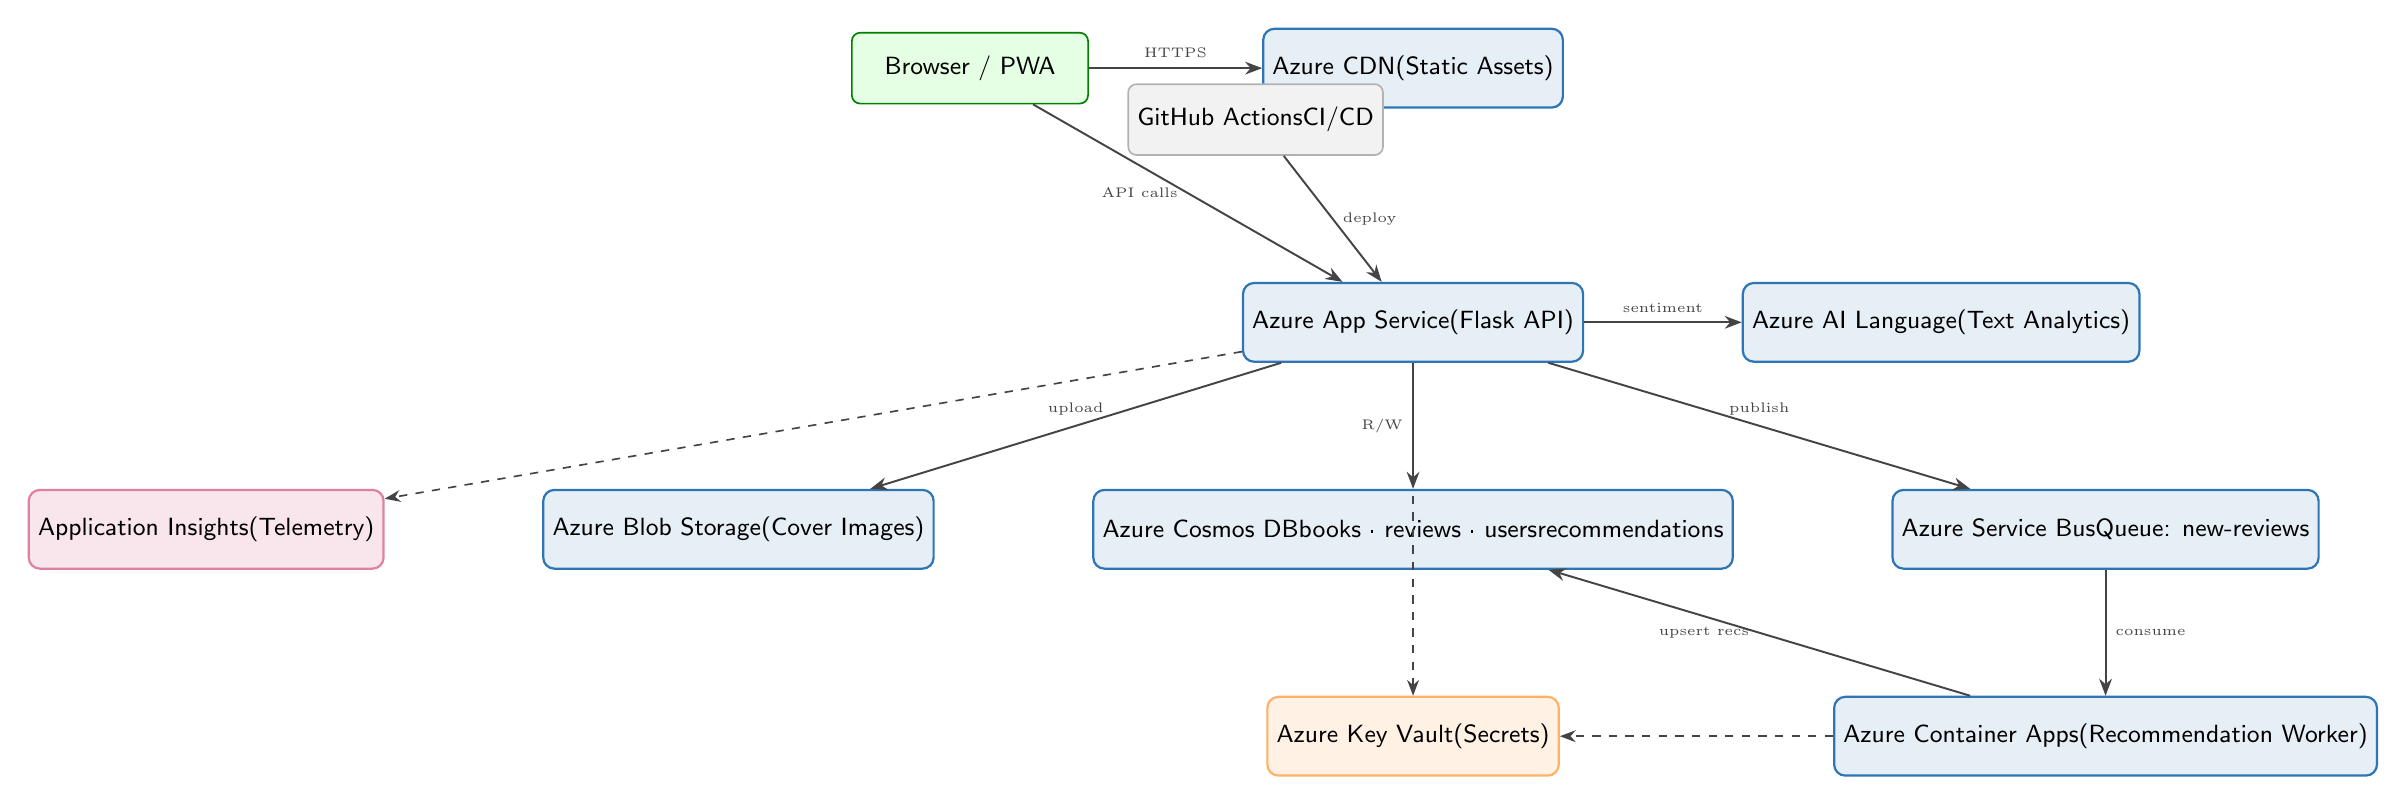
\begin{tikzpicture}[node distance=1.2cm and 1.6cm, >=Stealth,
                    every node/.style={font=\small\sffamily}]

  % ── Client ────────────────────────────────────────────
  \node[component, fill=green!10, draw=green!50!black, minimum width=3cm]
    (browser) {Browser / PWA};

  % ── CDN / Static ──────────────────────────────────────
  \node[azureservice, right=2.2cm of browser]
    (cdn) {Azure CDN\\(Static Assets)};

  % ── App Service ───────────────────────────────────────
  \node[azureservice, below=2.2cm of cdn]
    (appservice) {Azure App Service\\(Flask API)};

  % ── Azure AI ──────────────────────────────────────────
  \node[azureservice, right=2cm of appservice]
    (textanalytics) {Azure AI Language\\(Text Analytics)};

  % ── Cosmos DB ─────────────────────────────────────────
  \node[azureservice, below=1.6cm of appservice]
    (cosmos) {Azure Cosmos DB\\books · reviews · users\\recommendations};

  % ── Blob Storage ──────────────────────────────────────
  \node[azureservice, left=2cm of cosmos]
    (blob) {Azure Blob Storage\\(Cover Images)};

  % ── Service Bus ───────────────────────────────────────
  \node[azureservice, right=2cm of cosmos]
    (servicebus) {Azure Service Bus\\Queue: new-reviews};

  % ── Worker ────────────────────────────────────────────
  \node[azureservice, below=1.6cm of servicebus]
    (worker) {Azure Container Apps\\(Recommendation Worker)};

  % ── Key Vault ─────────────────────────────────────────
  \node[azureservice, fill=orange!10, draw=orange!60, below=1.6cm of cosmos]
    (keyvault) {Azure Key Vault\\(Secrets)};

  % ── App Insights ──────────────────────────────────────
  \node[azureservice, fill=purple!10, draw=purple!50, left=2cm of blob]
    (insights) {Application Insights\\(Telemetry)};

  % ── GitHub Actions ────────────────────────────────────
  \node[component, fill=gray!10, draw=gray!60,
        above=1.6cm of appservice, xshift=-2cm]
    (ghactions) {GitHub Actions\\CI/CD};

  % ── Arrows ────────────────────────────────────────────
  \draw[arrow] (browser) -- node[above, font=\tiny]{HTTPS} (cdn);
  \draw[arrow] (browser) -- node[left,  font=\tiny]{API calls} (appservice);
  \draw[arrow] (appservice) -- node[above, font=\tiny]{sentiment} (textanalytics);
  \draw[arrow] (appservice) -- node[left,  font=\tiny]{R/W} (cosmos);
  \draw[arrow] (appservice) -- node[above, font=\tiny]{upload} (blob);
  \draw[arrow] (appservice) -- node[above, font=\tiny]{publish} (servicebus);
  \draw[arrow] (servicebus) -- node[right, font=\tiny]{consume} (worker);
  \draw[arrow] (worker) -- node[left,  font=\tiny]{upsert recs} (cosmos);
  \draw[dashedarrow] (appservice) -- (keyvault);
  \draw[dashedarrow] (worker)     -- (keyvault);
  \draw[dashedarrow] (appservice) -- (insights);
  \draw[arrow] (ghactions) -- node[font=\tiny, right]{deploy} (appservice);

\end{tikzpicture}
\caption{BookVault – Azure Architecture Overview}
\label{fig:architecture}
\end{figure}

\section{Data Flow Description}

\begin{enumerate}[nosep]
  \item The \textbf{React SPA} is served as a PWA from \textbf{Azure CDN}; all API calls
    target the Flask backend on \textbf{Azure App Service} via HTTPS.
  \item On \textbf{review creation}, the API:
    \begin{enumerate}[nosep, label=\alph*.]
      \item Calls \textbf{Azure AI Language} for sentiment classification.
      \item Persists the review document in \textbf{Cosmos DB} (\texttt{reviews} container).
      \item Recomputes and caches the book's average rating in the \texttt{books} container.
      \item Publishes a JSON event to \textbf{Azure Service Bus}.
    \end{enumerate}
  \item The \textbf{Recommendation Worker} (Container Apps) polls the Service Bus queue,
    scores genre-peer books using a collaborative algorithm, and upserts personalised
    recommendation documents in Cosmos DB (\texttt{recommendations} container).
  \item \textbf{Azure Key Vault} provides secrets to both the API and the worker at runtime.
  \item \textbf{Application Insights} collects distributed traces and performance metrics.
  \item \textbf{GitHub Actions} runs the CI/CD pipeline on every push to \texttt{main}.
\end{enumerate}

% ============================================================
\chapter{Use-Case Diagrams}
% ============================================================

\section{Actors}

\begin{description}[nosep]
  \item[Guest] Unauthenticated visitor; read-only access.
  \item[Reader] Authenticated user; full platform participant.
  \item[Author/Publisher] Verified professional; accesses analytics dashboard.
  \item[Administrator] Platform staff; moderation and content management.
  \item[Recommendation Worker] Internal automated system (background process).
\end{description}

\section{Use-Case Diagram – Book Discovery \& Reviews}

\begin{figure}[H]
\centering
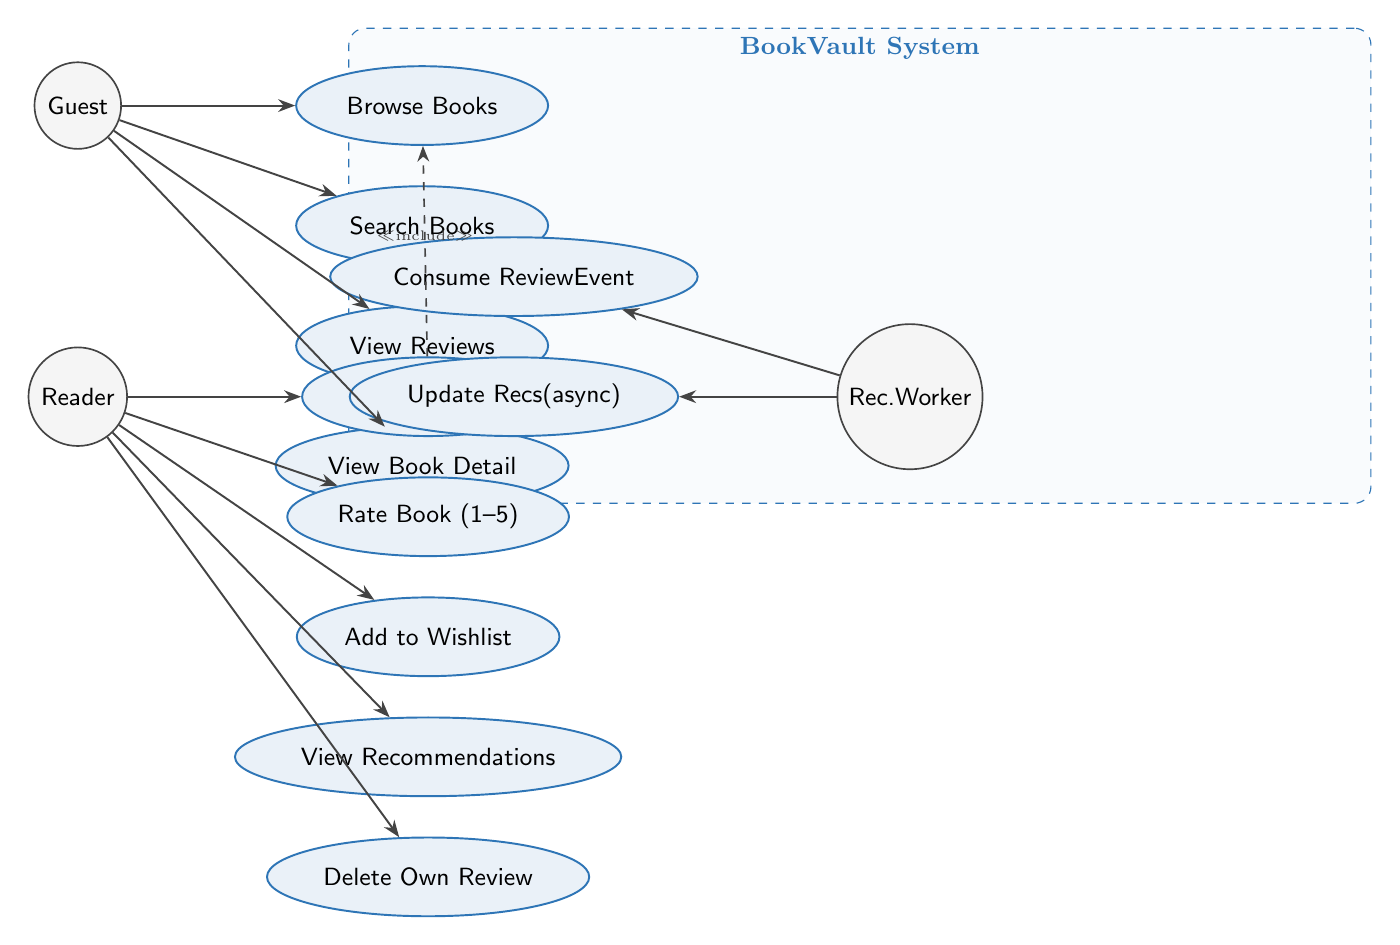
\begin{tikzpicture}[node distance=1.1cm and 2.4cm, >=Stealth,
                    every node/.style={font=\small\sffamily}]

  % ── Actors ────────────────────────────────────────────
  \node[actor] (guest) {Guest};
  \node[actor, below=2.5cm of guest] (reader) {Reader};
  \node[actor, right=9cm of reader] (worker) {Rec.\\Worker};

  % ── System boundary ───────────────────────────────────
  \begin{scope}[on background layer]
    \node[draw=accentblue, dashed, rounded corners=6pt,
          inner sep=12pt, fill=accentblue!3,
          fit=(guest)(reader)(worker),
          xshift=4.5cm]
      (boundary) {};
  \end{scope}
  \node[anchor=north, font=\bfseries\small, color=accentblue]
    at (boundary.north) {BookVault System};

  % ── Use cases – Guest ─────────────────────────────────
  \node[usecase, right=2.2cm of guest]
    (browsebooks) {Browse Books};
  \node[usecase, below=0.5cm of browsebooks]
    (searchbooks) {Search Books};
  \node[usecase, below=0.5cm of searchbooks]
    (viewreview)  {View Reviews};
  \node[usecase, below=0.5cm of viewreview]
    (viewbook)    {View Book Detail};

  % ── Use cases – Reader ────────────────────────────────
  \node[usecase, right=2.2cm of reader]
    (createreview)  {Create Review};
  \node[usecase, below=0.5cm of createreview]
    (ratebook)      {Rate Book (1–5)};
  \node[usecase, below=0.5cm of ratebook]
    (wishlist)      {Add to Wishlist};
  \node[usecase, below=0.5cm of wishlist]
    (viewrecs)      {View Recommendations};
  \node[usecase, below=0.5cm of viewrecs]
    (deletereview)  {Delete Own Review};

  % ── Use cases – Worker ────────────────────────────────
  \node[usecase, left=2cm of worker]
    (updaterecs)    {Update Recs\\(async)};
  \node[usecase, above=0.5cm of updaterecs]
    (consumequeue)  {Consume Review\\Event};

  % ── Arrows ────────────────────────────────────────────
  \draw[arrow] (guest)  -- (browsebooks);
  \draw[arrow] (guest)  -- (searchbooks);
  \draw[arrow] (guest)  -- (viewreview);
  \draw[arrow] (guest)  -- (viewbook);

  \draw[arrow] (reader) -- (createreview);
  \draw[arrow] (reader) -- (ratebook);
  \draw[arrow] (reader) -- (wishlist);
  \draw[arrow] (reader) -- (viewrecs);
  \draw[arrow] (reader) -- (deletereview);

  % reader includes guest capabilities (dashed «include»)
  \draw[dashedarrow] (createreview) -- node[above,font=\tiny]{«include»} (browsebooks);

  \draw[arrow] (worker) -- (consumequeue);
  \draw[arrow] (worker) -- (updaterecs);

\end{tikzpicture}
\caption{Use-Case Diagram – Book Discovery and Reviews}
\label{fig:usecase1}
\end{figure}

\section{Use-Case Diagram – User Profile \& Administration}

\begin{figure}[H]
\centering
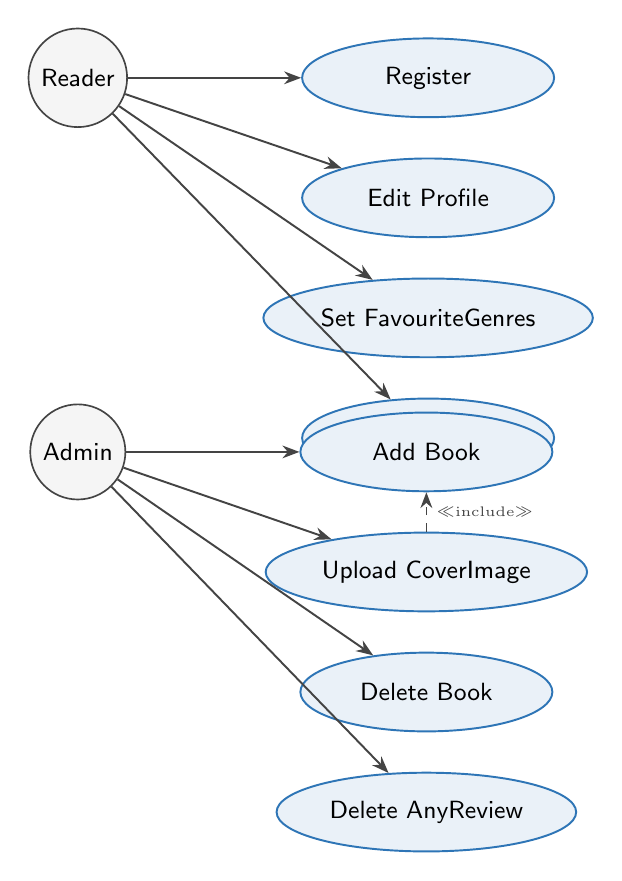
\begin{tikzpicture}[node distance=1cm and 2.2cm, >=Stealth,
                    every node/.style={font=\small\sffamily}]

  \node[actor] (reader) {Reader};
  \node[actor, below=3.5cm of reader] (admin) {Admin};

  \node[usecase, right=2.2cm of reader]
    (createuser)   {Register};
  \node[usecase, below=0.5cm of createuser]
    (updateprofile){Edit Profile};
  \node[usecase, below=0.5cm of updateprofile]
    (setgenres)    {Set Favourite\\Genres};
  \node[usecase, below=0.5cm of setgenres]
    (viewwishlist) {View Wishlist};

  \node[usecase, right=2.2cm of admin]
    (addbook)      {Add Book};
  \node[usecase, below=0.5cm of addbook]
    (uploadcover)  {Upload Cover\\Image};
  \node[usecase, below=0.5cm of uploadcover]
    (deletebook)   {Delete Book};
  \node[usecase, below=0.5cm of deletebook]
    (deletereview) {Delete Any\\Review};

  \draw[arrow] (reader) -- (createuser);
  \draw[arrow] (reader) -- (updateprofile);
  \draw[arrow] (reader) -- (setgenres);
  \draw[arrow] (reader) -- (viewwishlist);

  \draw[arrow] (admin)  -- (addbook);
  \draw[arrow] (admin)  -- (uploadcover);
  \draw[arrow] (admin)  -- (deletebook);
  \draw[arrow] (admin)  -- (deletereview);
  \draw[dashedarrow] (uploadcover) --
    node[right, font=\tiny]{«include»} (addbook);

\end{tikzpicture}
\caption{Use-Case Diagram – User Profile and Administration}
\label{fig:usecase2}
\end{figure}

% ============================================================
\chapter{API Documentation (OpenAPI 3.0)}
% ============================================================

\section{Overview}

The BookVault REST API follows the \textbf{OpenAPI 3.0.3} specification.
The canonical machine-readable file (\texttt{openapi.yaml}) is hosted on
\href{https://app.swaggerhub.com}{SwaggerHub} and should be considered the
source of truth. This chapter presents the human-readable summary.

\begin{infobox}
  \textbf{Base URL:} \texttt{https://api.bookvault.io/api}\\
  \textbf{Authentication:} Bearer JWT (Azure AD B2C) — header \texttt{Authorization: Bearer <token>}\\
  \textbf{Content-Type:} \texttt{application/json} (unless otherwise noted)\\
  \textbf{Versioning:} URL-path versioning (\texttt{/v1/}) planned for next major release.
\end{infobox}

\section{OpenAPI Specification Excerpt}

The following YAML is the \textit{complete, self-contained} OpenAPI document.
Paste it directly into \url{https://editor.swagger.io} or import it into SwaggerHub.

\begin{lstlisting}[style=yaml, caption={openapi.yaml – BookVault REST API}]
openapi: "3.0.3"
info:
  title: "BookVault API"
  description: |
    Social book-review platform API.
    Supports books, reviews, users, search and recommendations.
  version: "1.0.0"
  contact:
    name: "BookVault Team"
    email: "dev@bookvault.io"
  license:
    name: "MIT"

servers:
  - url: "https://api.bookvault.io/api"
    description: "Production"
  - url: "http://localhost:8000/api"
    description: "Local development"

tags:
  - name: books
    description: "Book catalogue management"
  - name: reviews
    description: "User reviews with sentiment"
  - name: users
    description: "User profiles and preferences"
  - name: search
    description: "Full-text search"
  - name: health
    description: "Service health"

# ── Security ────────────────────────────────────────────
components:
  securitySchemes:
    bearerAuth:
      type: http
      scheme: bearer
      bearerFormat: JWT

  schemas:
    Book:
      type: object
      required: [id, title, author, genre, year]
      properties:
        id:          { type: string, format: uuid }
        title:       { type: string, example: "Crime and Punishment" }
        author:      { type: string, example: "Fyodor Dostoevsky" }
        genre:       { type: string, example: "Classic" }
        year:        { type: integer, example: 1866 }
        description: { type: string }
        coverUrl:    { type: string, format: uri, nullable: true }
        avgRating:   { type: number, format: float, example: 4.5 }
        reviewCount: { type: integer, example: 120 }

    BookCreate:
      type: object
      required: [title, author, genre, year]
      properties:
        title:       { type: string }
        author:      { type: string }
        genre:       { type: string }
        year:        { type: integer }
        description: { type: string }

    Sentiment:
      type: object
      properties:
        label:
          type: string
          enum: [positive, neutral, negative, mixed, unknown]
        scores:
          type: object
          properties:
            positive: { type: number, format: float }
            neutral:  { type: number, format: float }
            negative: { type: number, format: float }

    Review:
      type: object
      required: [id, bookId, userId, rating, text, sentiment]
      properties:
        id:        { type: string, format: uuid }
        bookId:    { type: string, format: uuid }
        userId:    { type: string, format: uuid }
        rating:    { type: integer, minimum: 1, maximum: 5 }
        text:      { type: string }
        sentiment: { $ref: '#/components/schemas/Sentiment' }

    ReviewCreate:
      type: object
      required: [bookId, userId, rating, text]
      properties:
        bookId: { type: string, format: uuid }
        userId: { type: string, format: uuid }
        rating: { type: integer, minimum: 1, maximum: 5 }
        text:   { type: string, minLength: 10 }

    User:
      type: object
      required: [id, email]
      properties:
        id:              { type: string, format: uuid }
        email:           { type: string, format: email }
        displayName:     { type: string }
        favoriteGenres:  { type: array, items: { type: string } }
        readBookIds:     { type: array, items: { type: string } }
        wishlistBookIds: { type: array, items: { type: string } }

    Error:
      type: object
      properties:
        error: { type: string }
        code:  { type: integer }

  responses:
    NotFound:
      description: "Resource not found"
      content:
        application/json:
          schema: { $ref: '#/components/schemas/Error' }
    BadRequest:
      description: "Validation error"
      content:
        application/json:
          schema: { $ref: '#/components/schemas/Error' }

# ── Paths ───────────────────────────────────────────────
paths:

  # HEALTH
  /health:
    get:
      tags: [health]
      summary: "Health check"
      responses:
        "200":
          description: "OK"
          content:
            application/json:
              schema:
                type: object
                properties:
                  status:  { type: string, example: "ok" }
                  service: { type: string, example: "BookVault API" }

  # BOOKS
  /books:
    get:
      tags: [books]
      summary: "List books"
      parameters:
        - name: genre
          in: query
          schema: { type: string }
        - name: limit
          in: query
          schema: { type: integer, default: 20, maximum: 100 }
        - name: offset
          in: query
          schema: { type: integer, default: 0 }
      responses:
        "200":
          description: "Array of books"
          content:
            application/json:
              schema:
                type: array
                items: { $ref: '#/components/schemas/Book' }
    post:
      tags: [books]
      summary: "Create a book"
      security: [{ bearerAuth: [] }]
      requestBody:
        required: true
        content:
          application/json:
            schema: { $ref: '#/components/schemas/BookCreate' }
      responses:
        "201":
          description: "Book created"
          content:
            application/json:
              schema: { $ref: '#/components/schemas/Book' }
        "400": { $ref: '#/components/responses/BadRequest' }

  /books/{bookId}:
    parameters:
      - name: bookId
        in: path
        required: true
        schema: { type: string, format: uuid }
    get:
      tags: [books]
      summary: "Get a book"
      responses:
        "200":
          description: "Book object"
          content:
            application/json:
              schema: { $ref: '#/components/schemas/Book' }
        "404": { $ref: '#/components/responses/NotFound' }
    patch:
      tags: [books]
      summary: "Update a book"
      security: [{ bearerAuth: [] }]
      requestBody:
        required: true
        content:
          application/json:
            schema: { $ref: '#/components/schemas/BookCreate' }
      responses:
        "200":
          description: "Updated book"
          content:
            application/json:
              schema: { $ref: '#/components/schemas/Book' }
        "404": { $ref: '#/components/responses/NotFound' }
    delete:
      tags: [books]
      summary: "Delete a book"
      security: [{ bearerAuth: [] }]
      responses:
        "204": { description: "Deleted" }
        "404": { $ref: '#/components/responses/NotFound' }

  /books/{bookId}/cover:
    put:
      tags: [books]
      summary: "Upload cover image"
      security: [{ bearerAuth: [] }]
      parameters:
        - name: bookId
          in: path
          required: true
          schema: { type: string, format: uuid }
      requestBody:
        required: true
        content:
          multipart/form-data:
            schema:
              type: object
              properties:
                cover:
                  type: string
                  format: binary
      responses:
        "200":
          description: "Cover URL"
          content:
            application/json:
              schema:
                type: object
                properties:
                  coverUrl: { type: string, format: uri }
        "415": { description: "Unsupported media type" }

  # REVIEWS
  /reviews:
    post:
      tags: [reviews]
      summary: "Create a review (triggers sentiment analysis)"
      security: [{ bearerAuth: [] }]
      requestBody:
        required: true
        content:
          application/json:
            schema: { $ref: '#/components/schemas/ReviewCreate' }
      responses:
        "201":
          description: "Review with sentiment"
          content:
            application/json:
              schema: { $ref: '#/components/schemas/Review' }
        "400": { $ref: '#/components/responses/BadRequest' }

  /reviews/book/{bookId}:
    get:
      tags: [reviews]
      summary: "List reviews for a book"
      parameters:
        - name: bookId
          in: path
          required: true
          schema: { type: string, format: uuid }
        - name: limit
          in: query
          schema: { type: integer, default: 20 }
        - name: offset
          in: query
          schema: { type: integer, default: 0 }
      responses:
        "200":
          description: "Array of reviews"
          content:
            application/json:
              schema:
                type: array
                items: { $ref: '#/components/schemas/Review' }

  /reviews/{reviewId}:
    parameters:
      - name: reviewId
        in: path
        required: true
        schema: { type: string, format: uuid }
    get:
      tags: [reviews]
      summary: "Get a single review"
      responses:
        "200":
          description: "Review"
          content:
            application/json:
              schema: { $ref: '#/components/schemas/Review' }
        "404": { $ref: '#/components/responses/NotFound' }
    delete:
      tags: [reviews]
      summary: "Delete a review"
      security: [{ bearerAuth: [] }]
      responses:
        "204": { description: "Deleted" }
        "404": { $ref: '#/components/responses/NotFound' }

  # USERS
  /users:
    post:
      tags: [users]
      summary: "Create user profile"
      requestBody:
        required: true
        content:
          application/json:
            schema:
              type: object
              required: [email]
              properties:
                email:          { type: string, format: email }
                displayName:    { type: string }
                favoriteGenres: { type: array, items: { type: string } }
      responses:
        "201":
          description: "Created user"
          content:
            application/json:
              schema: { $ref: '#/components/schemas/User' }

  /users/{userId}:
    parameters:
      - name: userId
        in: path
        required: true
        schema: { type: string, format: uuid }
    get:
      tags: [users]
      summary: "Get user profile"
      security: [{ bearerAuth: [] }]
      responses:
        "200":
          description: "User"
          content:
            application/json:
              schema: { $ref: '#/components/schemas/User' }
        "404": { $ref: '#/components/responses/NotFound' }
    patch:
      tags: [users]
      summary: "Update user profile"
      security: [{ bearerAuth: [] }]
      requestBody:
        required: true
        content:
          application/json:
            schema:
              type: object
              properties:
                displayName:    { type: string }
                favoriteGenres: { type: array, items: { type: string } }
      responses:
        "200":
          description: "Updated user"
          content:
            application/json:
              schema: { $ref: '#/components/schemas/User' }

  /users/{userId}/wishlist/{bookId}:
    put:
      tags: [users]
      summary: "Add book to wishlist"
      security: [{ bearerAuth: [] }]
      parameters:
        - name: userId
          in: path
          required: true
          schema: { type: string, format: uuid }
        - name: bookId
          in: path
          required: true
          schema: { type: string, format: uuid }
      responses:
        "200":
          description: "Updated wishlist"
          content:
            application/json:
              schema:
                type: object
                properties:
                  wishlist:
                    type: array
                    items: { type: string }

  # SEARCH
  /search:
    get:
      tags: [search]
      summary: "Search books by title, author or description"
      parameters:
        - name: q
          in: query
          required: true
          schema: { type: string, minLength: 1 }
          description: "Search query (case-insensitive)"
        - name: limit
          in: query
          schema: { type: integer, default: 10, maximum: 50 }
      responses:
        "200":
          description: "Matching books"
          content:
            application/json:
              schema:
                type: array
                items: { $ref: '#/components/schemas/Book' }
\end{lstlisting}

\section{Functionality Flow Documentation}

\subsection{Flow 1 – Create Review with Sentiment}

\begin{figure}[H]
\centering
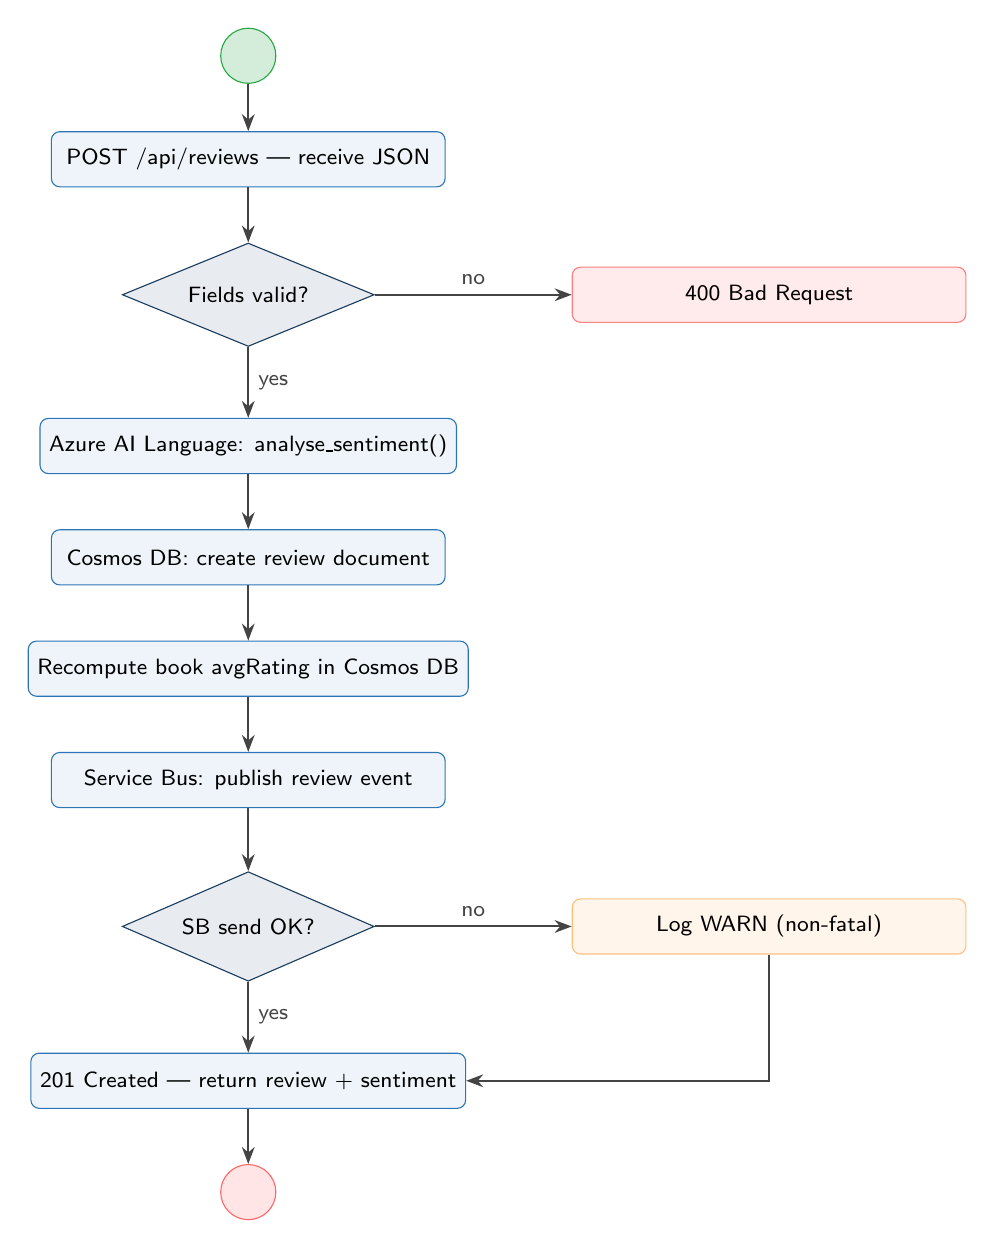
\begin{tikzpicture}[
  node distance=0.9cm,
  every node/.style={font=\footnotesize\sffamily},
  box/.style={rectangle, rounded corners=3pt, draw=accentblue, fill=accentblue!8,
              minimum width=5cm, minimum height=0.7cm, text centered},
  decision/.style={diamond, draw=primaryblue, fill=primaryblue!10,
                   minimum width=3.2cm, minimum height=0.8cm, text centered,
                   aspect=2},
  start/.style={circle, draw=codegreen, fill=codegreen!20, minimum size=0.7cm},
  stop/.style={circle, draw=red!60, fill=red!10, minimum size=0.7cm},
]
  \node[start] (start) {};
  \node[box, below=0.6cm of start]
    (recv)   {POST /api/reviews — receive JSON};
  \node[decision, below=0.7cm of recv]
    (valid)  {Fields valid?};
  \node[box, right=2.5cm of valid, fill=red!8, draw=red!50]
    (err400) {400 Bad Request};
  \node[box, below=0.9cm of valid]
    (sent)   {Azure AI Language: analyse\_sentiment()};
  \node[box, below=0.7cm of sent]
    (store)  {Cosmos DB: create review document};
  \node[box, below=0.7cm of store]
    (rating) {Recompute book avgRating in Cosmos DB};
  \node[box, below=0.7cm of rating]
    (pub)    {Service Bus: publish review event};
  \node[decision, below=0.8cm of pub]
    (sbfail) {SB send OK?};
  \node[box, right=2.5cm of sbfail, fill=orange!8, draw=orange!50]
    (warn)   {Log WARN (non-fatal)};
  \node[box, below=0.9cm of sbfail]
    (resp)   {201 Created — return review + sentiment};
  \node[stop, below=0.7cm of resp] (stop) {};

  \draw[arrow] (start)  -- (recv);
  \draw[arrow] (recv)   -- (valid);
  \draw[arrow] (valid)  -- node[right]{yes} (sent);
  \draw[arrow] (valid)  -- node[above]{no}  (err400);
  \draw[arrow] (sent)   -- (store);
  \draw[arrow] (store)  -- (rating);
  \draw[arrow] (rating) -- (pub);
  \draw[arrow] (pub)    -- (sbfail);
  \draw[arrow] (sbfail) -- node[right]{yes} (resp);
  \draw[arrow] (sbfail) -- node[above]{no}  (warn);
  \draw[arrow] (warn)   |- (resp);
  \draw[arrow] (resp)   -- (stop);
\end{tikzpicture}
\caption{Flow 1 – Review Creation with Sentiment Analysis}
\end{figure}

\subsection{Flow 2 – Recommendation Update (Background Worker)}

\begin{enumerate}[nosep]
  \item Worker polls \texttt{Azure Service Bus} queue (\texttt{new-reviews}).
  \item For each message, deserialise JSON event: \texttt{\{bookId, userId, rating, sentiment\}}.
  \item Query Cosmos DB for the book's \texttt{genre}.
  \item Query all books in the same genre; compute score:
    \[
      \text{score}_i = \overline{r}_i \cdot \log_2\!\left(n_i + 1\right)
    \]
    where $\overline{r}_i$ is the book's average rating and $n_i$ its review count.
  \item Sort by score descending; keep top 10.
  \item Upsert document \texttt{\{userId, genre, recommendations: [\ldots]\}} in
    \texttt{recommendations} container.
  \item \texttt{complete\_message()} on success; \texttt{abandon\_message()} on exception
    (message returns to queue for retry).
\end{enumerate}

\subsection{Flow 3 – Cover Image Upload}

\begin{enumerate}[nosep]
  \item Client sends \texttt{PUT /api/books/\{bookId\}/cover} as \texttt{multipart/form-data}.
  \item API validates MIME type (\texttt{image/jpeg}, \texttt{image/png}, \texttt{image/webp}).
  \item Book is fetched from Cosmos DB; 404 if absent.
  \item Blob is uploaded to Azure Blob Storage container \texttt{book-covers} with
    \texttt{overwrite=True}; blob name: \texttt{\{bookId\}.\{ext\}}.
  \item \texttt{coverUrl} field on the book document is updated in Cosmos DB.
  \item Response: \texttt{200 \{"coverUrl": "https://..."\}}.
\end{enumerate}

\subsection{Flow 4 – Full-Text Search}

\begin{enumerate}[nosep]
  \item Client sends \texttt{GET /api/search?q=\{query\}\&limit=\{n\}}.
  \item Query string is lower-cased; empty string returns \texttt{[]}.
  \item Cosmos DB SQL query uses \texttt{CONTAINS(LOWER(c.field), @q)} on
    \texttt{title}, \texttt{author}, and \texttt{description}.
  \item Results are returned ordered by Cosmos DB's default index scan order.
  \item \textit{Production note:} For relevance ranking and fuzzy matching, replace with
    \textbf{Azure Cognitive Search} index pointed at the same Cosmos DB change feed.
\end{enumerate}

% ============================================================
\chapter{Conclusions \& Roadmap}
% ============================================================

\section{Summary}

BookVault applies a proven social-media product model (Letterboxd) to the global reading
market, differentiating through AI-enriched reviews, an open REST API, and a modern cloud
architecture built entirely on Microsoft Azure.  The current implementation covers the
core CRUD operations, sentiment analysis, and asynchronous recommendations.

\section{Planned Roadmap}

\begin{table}[H]
  \centering
  \caption{Roadmap (12-month horizon)}
  \begin{tabularx}{\textwidth}{C{1.5cm} L{3.5cm} X}
    \toprule
    \textbf{Quarter} & \textbf{Feature} & \textbf{Details} \\
    \midrule
    Q1 & Authentication & Azure AD B2C; JWT-secured endpoints; social login (Google, Facebook) \\
    Q1 & Social graph   & Follow/unfollow users; activity feed \\
    Q2 & PWA            & Service Worker; offline reading log; push notifications \\
    Q2 & Azure Cognitive Search & Replace CONTAINS queries; faceted search; fuzzy matching \\
    Q3 & Mobile apps    & React Native (iOS \& Android); shared business logic \\
    Q3 & Author dashboard & Publisher analytics: sentiment trends, reader demographics \\
    Q4 & Reading goals  & Annual challenge; streak tracking; shareable graphics (viral loop) \\
    Q4 & Localisation   & Romanian translation; multi-language sentiment analysis \\
    \bottomrule
  \end{tabularx}
\end{table}

\section{Known Limitations}

\begin{itemize}[nosep]
  \item \textbf{Search quality:} Cosmos DB \texttt{CONTAINS} is case-insensitive substring
    match only; no relevance ranking or typo tolerance.
  \item \textbf{Authentication:} Not yet implemented; all endpoints are effectively public.
  \item \textbf{Recommendation algorithm:} Score function is naïve (no user-preference
    weighting, no collaborative filtering across users).
  \item \textbf{Partition key design:} Partition on \texttt{/genre} for books causes
    hot partitions for popular genres; consider hashed partition in production.
\end{itemize}

% ── Bibliography (optional placeholder) ───────────────────
\begin{thebibliography}{9}
  \bibitem{openapi}
    OpenAPI Initiative, \textit{OpenAPI Specification 3.0.3},
    \url{https://spec.openapis.org/oas/v3.0.3}, 2021.
  \bibitem{cosmosdb}
    Microsoft, \textit{Azure Cosmos DB Documentation},
    \url{https://learn.microsoft.com/azure/cosmos-db/}, 2024.
  \bibitem{textanalytics}
    Microsoft, \textit{Azure AI Language – Sentiment Analysis},
    \url{https://learn.microsoft.com/azure/ai-services/language-service/sentiment-opinion-mining/overview}, 2024.
  \bibitem{servicebus}
    Microsoft, \textit{Azure Service Bus Documentation},
    \url{https://learn.microsoft.com/azure/service-bus-messaging/}, 2024.
  \bibitem{goodreads}
    Goodreads LLC, \textit{About Goodreads},
    \url{https://www.goodreads.com/about/us}, 2024.
  \bibitem{storygraph}
    The StoryGraph, \textit{About},
    \url{https://www.thestorygraph.com}, 2024.
  \bibitem{grandview}
    Grand View Research, \textit{Book Market Size, Share \& Trends Analysis Report},
    San Francisco, 2023.
\end{thebibliography}

\end{document}
\end antml:parameter>
